\documentclass[10pt,twocolumn]{article} 
\usepackage{simpleConference}
\usepackage{times}
\usepackage{graphicx}
\graphicspath{ {images/} }
\usepackage{amssymb}
\PassOptionsToPackage{hyphens}{url}\usepackage{hyperref}
\begin{document}

\title{Subterranean WiFi (SWIFT)}

\author{Amy Reed, Kristina Hager\\
Mobile Computing EE382V\\
University of Texas at Austin\\
\\
}

\maketitle
\thispagestyle{empty}

\begin{abstract}
	We will consider a common problem scientists face when doing research in caves 
	involving sensors and associated data loggers.
	The most common method of retrieving this data from the data loggers is via a human entering 
	the cave, traveling to the collection site, and manually retrieving it. 
	This method is very slow, inconvenient, and sometimes dangerous.
	We propose a new means of data retrieval from cave sensors which is to automatically 
	ferry data back to the surface using WiFi Direct enabled devices. 
	We will focus on two key questions in this paper regarding the potential of the WiFi Direct technology for this application.
	First, we will create an application to determine the achievable range of the WiFi Direct technology in a cave environment.
	Next, we will create a prototype application for ferrying data using WiFi Direct as provided by the Android platform. 
	We will outline the implementation of both applications and describe any nuances associated with the current Android 
	support for WiFi Direct.
\end{abstract}

\tableofcontents

\section{Introduction}

\subsection{Usage of Sensors and Data Loggers in Caves}
\label{sec:Usage of Sensors and Data Loggers in Caves}
Many types of scientists such as geologists, hydrogeologists, climatologists and more conduct research in the interior of caves. 
These scientists are usually looking for information about the cave's microclimate and changes to the caves microclimate. 
For example, in \cite{wong2010}, the scientists are interested in monitoring changes in cave air CO$_2$ levels in response to brush clearing in areas above the cave. 

Caves present a wide variety of size and shape of passage and climate. 
% kh - Out of place.. might fit in better elsewhere
% Since power management is especially important for mobile devices WiFi direct includes power management mechanisms that can reduce power consumption for devices regardless of role.
For example, Son Doong Cave in Thailand has a large room that is over five kilometers long, 200 meters high and 150 meters wide \cite{sondoong}.
However, in the cave we visited for our research, most passages are just large enough to permit an adult to crawl through them.
Some rooms in this cave do allow an adult to stand up in just a few spots.

Most caves are difficult and dangerous to travel through to some degree and data loggers are often placed deep in the cave.
Therefore, a researcher expends a great deal of time, logistics and even risk to her life when she needs to access her sensors and the data logger attached to the sensor.
Also, most cave climates have nearly 100\% humidity at all times and some caves flood or in general have conditions that make sensors and data loggers prone to failure.
When a sensor or data logger fails, the scientist loses a great deal of data which adds to the difficulty of cave research.
Therefore, cave researchers are interested in mechanisms that would make their data easier to access and available in a more timely manner.

\begin{figure*}[t]
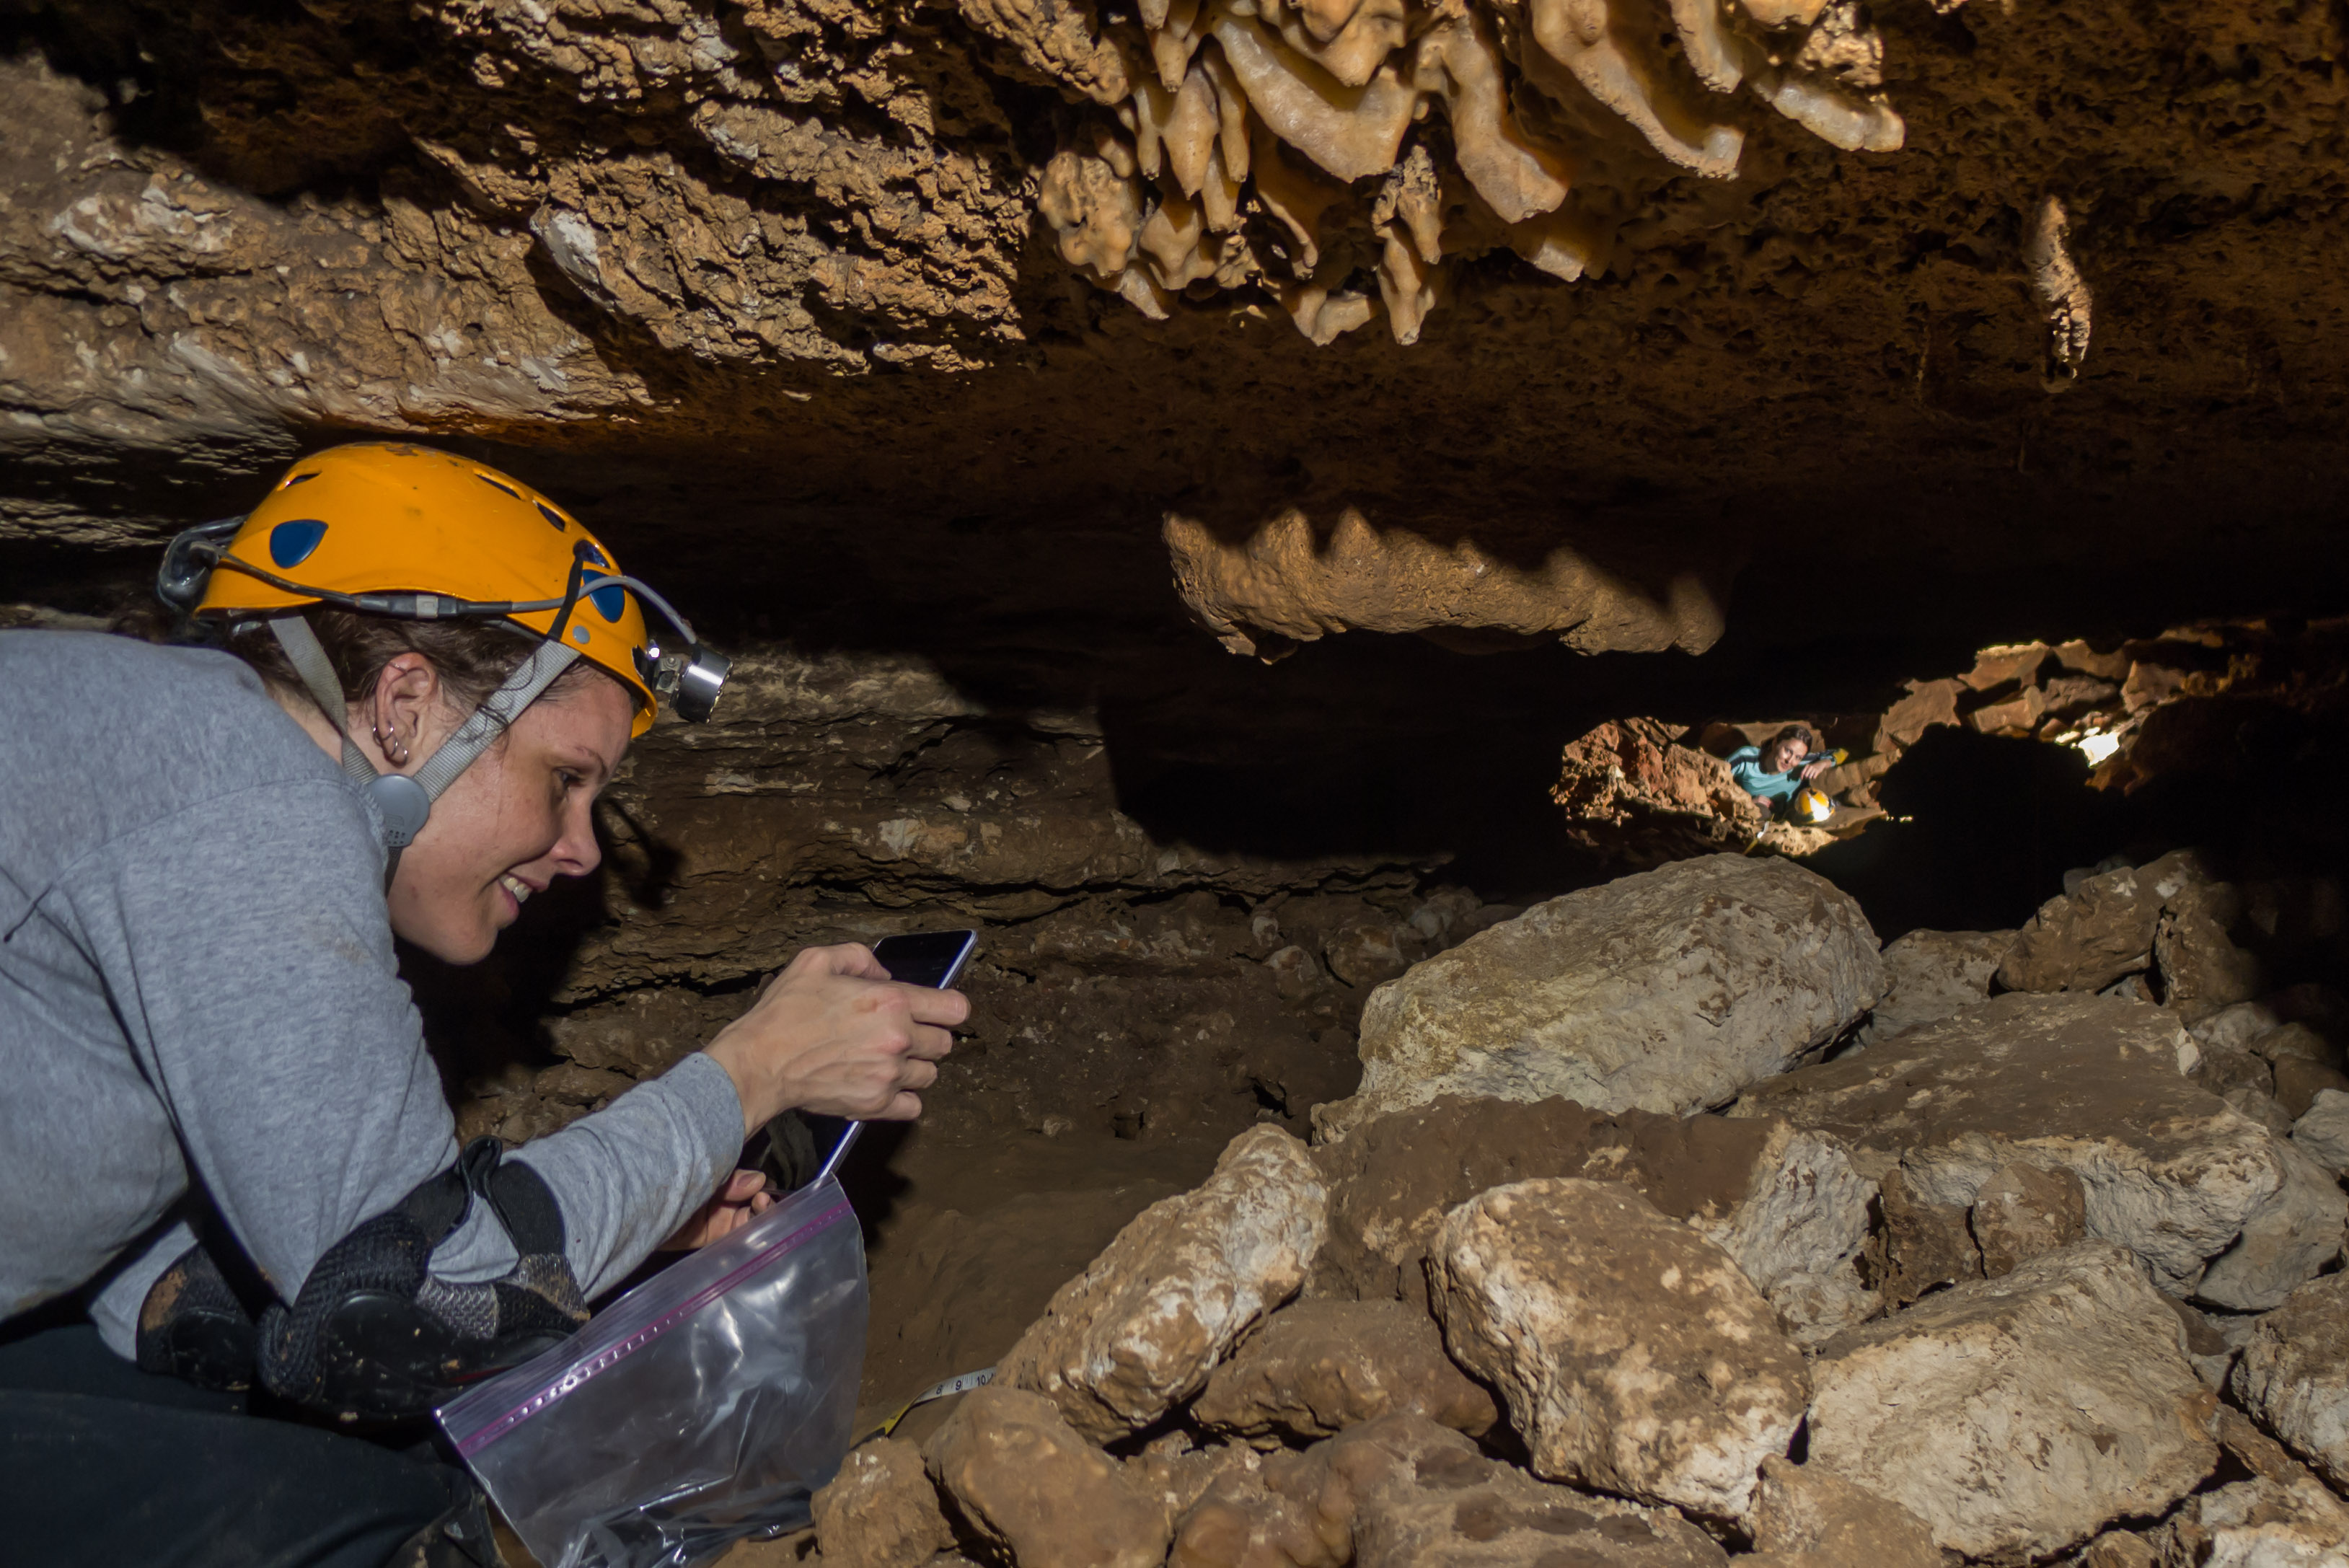
\includegraphics[width=\textwidth]{cavewifi2}
\caption{Testing WiFi Direct range in Whirlpool cave. \textit{Image courtesy of David Ochel.}}
\end{figure*}

\subsection{Outline of WiFi Direct Investigation}
\label{sec:Outline}
We propose here to automatically ferry data collected by a sensor from within a cave back to the surface using WiFi Direct enabled devices. 
% This technology is now common in many mobile devices.
This would be a far more convenient, effective, and safe mechanism for data retrieval versus current techniques.  
The WiFi Direct standard provides infrastructure mechanisms for discovery, addressing, and security which 
provides a simple and power effective means of setting up the network and transferring data. 

We will focus on two key questions in this paper regarding the potential of the WiFi Direct technology for this application.
First, we will investigate the range of the WiFi Direct technology in a cave environment.
WiFi Direct theoretically provides a range of up to 200m which is greater than that of Bluetooth technology. 
However, we would like to determine the potential range of WiFi Direct specifically in a cave environment which has different characteristics from a usual surface environment. 
Next, we will investigate how to ferry data from device to device using WiFi Direct as provided by the Android platform. 

However, the still nascent implementation of the WiFi Direct standard poses some limitations for our use case.
Since the data will need to travel from device to device beyond the range of a single wifi direct group, 
each device will need to participate in one or two groups. 
The current implementation of WiFi Direct on Android devices does not allow a device to be simultaneously connected to two WiFi Direct groups.
Therefore, our prototype application will manage the disconnect from one group and connection to the next group automatically.

In addition, the current Wifi Protected Setup (WPS) implementation requires the human user of the device to approve any new connections.
However, once a device has gained user permission once to a join a group, the Android platform "remembers" that permission and allows the device to automatically rejoin that group.
Since we want our devices to be able to operate autonomously, we will show how to accommodate the approval issue by pre-configuring the devices in their planned sequence.
 
For the first phase of this project, we created a prototype application for Android devices. 
We used this application to test the ability to make WiFi Direct connections within Whirlpool Cave, a popular cave in south Austin with a variety of passage characteristics. 
The ultimate goal of this initial application and the cave excursion is to determine if the range and bandwidth of WiFi Direct is sufficient to support passing messages out of the cave.
The results of this initial testing showed that WiFi Direct had significant range in areas of the cave where direct line of sight was achievable between devices.
Just as a note, in typical deployment environments, wifi signals do not require direct line of sight as they can travel through common building materials.
However, the radio waves of wifi signals cannot travel through substances like rock or concrete.
We will discuss these experiments in Section~\ref{sec:WiFi Direct Range in a Cave}.

For the second phase of the project, we developed a second Android application to demonstrate how to pass a sample data file from device to device in a manner similar to how data would be ferried out of a cave.
Ultimately the second application successfully demonstrates that passing data from peer to peer using WiFi Direct is achievable. 
In the development of this application, we developed code to manage a device's participation in multiple WiFi Direct groups.
We also spent considerable effort managing timing, connection, and synchronization issues between the devices.
We explain these issues later in the paper, and we consider these issues to indicate areas of future work for middleware solutions
such as the Android platform.

% We have not yet finished our research project. 
% This paper serves to cover the progress that has been made thus far into answering the questions outlined in this introduction. 


\section{Related Work}
\label{sec:Related}
Cave explorers and researchers need in cave communication systems in order to carry out complex group tasks such as expedition management, rescues, or photography projects.

Wired telephone technology is popular with expedition and rescue teams because they are simple and robust \cite{cavecomm}.
However, one major drawback of wire based systems is that the wire must be carefully laid along the cave passage. 
The wires themselves are heavy to carry and expensive.
Also, if the wire is broken somewhere along the line, then the entire system will not work.
Therefore, the drawbacks of wired telephone technology are the cost and weight of the wire and fragility of the system.

The APRS Cave-Link system is capable of sending text based messages via VHF/UHF walkie talkies or relay boxes placed along a cave passage.
In their experiments in a large cave, the average hop length was an average of 390' and 440' for VHF and UHF respectively.
The advantages of this system over wired systems is that the radio units and relay boxes are approximately hand-sized and are relatively lightweight.
The authors were using the system to essentially send text messages and did not address the general data capacity of the system \cite{cavelink}.

In Postojna Cave in Slovenia, a research team created a system for delay tolerant automatic data transfer from environmental monitoring systems deep in the cave.
Postojna Cave has a train to ferry tourists 2km into the cave.
Their system treats this train as a data mule by equipping it with a wifi enabled computer which connects to monitoring stations inside the cave as the train passes by \cite{postojna2014}.
Overall, this is a very interesting approach. 
However, it requires a cave with regular traffic of some type to act as the data mule.

Moore, et al \cite{moore2012} considers using autonomous mobile radio nodes to connect a base station to a leader node via wifi in tunnel exploration. 
Tunnel environments share some similarities with cave environments in that the passages usually consist of rough, concrete (rock-like) walls with straighter, longer passages of more consistent dimensions. 
Therefore, their experiments with wifi signal attenuation in the tunnel environment give us useful data to use in predicting range possibilities in a cave environment.

\section{WiFi Direct and Android Support}

\subsection{WiFi Direct Overview}
\label{sec:WifiD Overview}
Today, wireless connectivity is largely taken for granted. 
There are still a few circumstances that remind us that the Internet and general network connectivity are not guaranteed. 
% Whether due to physical or technological constraints, occasionally device connectivity cannot be achieved. 
The WiFi Direct standard is one means of potentially filling that gap. 
In some use cases, broader connectivity to infrastructure is not required and there is value to simple device to device communication. 
This is WiFi Direct's niche, those circumstances where a broader infrastructure is either unavailable or unnecessary, and device to device communication is needed.

WiFi Direct is a standard developed by the WiFi Alliance which provides a mechanism for peer to peer communication in the absence of a dedicated wireless infrastructure. 
This standard has several benefits, first and foremost being that it does not require a dedicated wireless access point \cite{whywifid}
, therefore users don't have worry about a DHCP server or other infrastructure pieces to enable their communication. 
In addition, this standard runs on typical wireless hardware found in all mobile devices, and is supported by most of the major mobile platforms such as Android 4.0, IOS 7, Blackberry, Windows 8, and even Xbox. 
Speed and range for WiFi Direct are those of typical WiFi devices and can operate at 250 Mbps and up to 200 meters depending on the environment. 
Security for WiFi direct utilizes WPS and WPA-2 to ensure security of the communications over the peer to peer network. 
Since power management is especially important for mobile devices WiFi direct includes power management mechanisms that can reduce power consumption for devices regardless of role.
All of these benefits makes WiFi Direct an ideal consideration to utilize as the technology for ferrying data from an underground cave.

The basic concepts of WiFi Direct are as follows. 
At the core of WiFi Direct is the WiFi Direct Group. 
The WiFi Direct group basically functions as an infrastructure basic service set(BSS). 
All components that can connect into a wireless medium in a network are referred to as stations. 
The BSS is a set of all stations that can communicate with each other. 
An infrastructure BSS includes both access points and stations in a wireless connection scenario.\cite{wirelesslanwiki}
All WiFi Direct devices must be capable of becoming the group owner. 
Within a group, a single device takes on this role.
 
The Group Owner is responsible for controlling which devices are allowed to join a group, when the group is started and terminated, BSS functionality, WPS Internal Registrar functionality, and communication between Clients in the Group. 
The Group owner decides if the group is temporary or persistent, a persistent group may be formed again without reinitiating WPS.
Group owners may optionally provide features such as simultaneous (concurrent) connection with an infrastructure network and sharing of that infrastructure connection. 
In addition to being able to execute the group owner role, WiFi Direct devices must also be capable of group ownership negotiation, discovery, and power management functions.
 
Devices adhering to the standard enter into a discovery phase where peers within range are found. 
Once a list of peers is retrieved, devices wishing to connect may either form a new  WiFi Direct group or connect to an existing group. 
As part of the group formation process, the devices wishing to connect establish which device will become the group owner.

A device obtains the role of group owner through one of three mechanisms: Standard, Autonomous, or Persistent. 
With Standard, devices negotiate to become the group owner.
With Persistent, a device identifies that a peer has been established as part of a past group. 
The group can be reformed, and the formation process can occur with a significantly reduced WPS phase because credentials for the devices have been stored.
With Autonomous, a device declares itself a group owner without involvement from any other peer devices. 
As part of providing the BSS functionality for the network, the group owner is responsible for providing DHCP addresses to devices on the network.
Data I/O can be handled via typical TCP/IP sockets, using the DHCP address provided by the group owner once the group is established\cite{wifiwhitepaper}.

As part of the connection process, WPS is used to obtain credentials and authenticate the WiFi Direct device.  
This type of security requires user intervention in the form of the user either pushing a button or providing a PIN on the device.
To execute WPS, the group owner generates and issues the security keys to other devices in the group. 
WPS, which is based on WPA-2 security, uses Advanced Encryption Standard (AES)-CCMP as cipher, and a randomly generated Pre-Shared Key (PSK) for mutual authentication\cite{wifiwhitepaper}.
After this part of the process devices disconnect and reconnect using their new authentication credentials.
With persistent groups, since credentials have been stored, the previous process of establishing authentication can be skipped and the two devices can use their credentials to connect.

\section{Android APIs For WiFi Direct}
\label{sec:Android APIs For WiFi Direct}
For this project, we used the Android platform to evaluate WiFi Direct for the Swift use case.
Starting with Android 4.0(API 14 and higher), Android provides three main areas within their API to support WiFi Direct.
These are the WiFi manager, Listeners, and Intents.
The WiFi manager class provides methods to allow you to interact with the Wi-Fi hardware on your device to do things like discover and connect to peers. 
Listeners allow you to be notified of the success or failure of WifiP2pManager method calls. 
Intents notify you of specific events detected by the Wi-Fi P2P framework, such as a dropped connection or a newly discovered peer. 
Actual data transfer between devices are handled by standard TCP/IP socket objects and I/O operations.
Android devices making use of the WiFi Direct functionality are required to request application permissions for: ACCESS\_WIFI\_STATE, CHANGE\_WIFI\_STATE, ACCESS\_NETWORK\_STATE, CHANGE\_NETWORK\_STATE, and INTERNET. \cite{androidoverview}

An application wishing to utilize WiFi Direct should implement several components to handle discovery and connectivity to peer devices.
First, the application must setup a Broadcast Receiver. 
A broadcast receiver allows you to receive intents broadcast by the Android system, in this case the application should respond to Wi-Fi peer to peer intents.
The broadcast receiver should implement necessary function calls to handle these intents in the Broadcast Receiver's "onReceive()" method.
The application will register the broadcast receiver and intent filter for the WiFi peer to peer events.
The application also should set up a Peer to Peer manager. 
The peer to peer manager, or "WifiP2pManager" class will be instantiated in the application, and used to create a channel which will be passed to the broadcast receiver.x

To discover peer devices, the "discoverPeers()" method is called from the peer to peer manager created for the application.
Discovery is asynchronous, so an intent is used to notify the application when discovered peers are available.
Once the application receives notification of available peers, the peer to peer manager can be queried for the list of available peers by calling the "requestPeers()" function. 
This function call is also asynchronous and the function "onPeersAvailable()" is executed when the "requestPeers()" function succeeds. 
This provides a list of WifiP2pDevice devices which can be used to establish a connection. \cite{androidp2p}

When a device is selected for a connection, the wifi peer to peer manager is used to call the "connect()" function to establish the connection to the device. 
This method is passed a WifiP2pConfig object which can be assigned parameters from the WifiP2pDevice such as the device's address.
The "connect()" method is another asynchronous call. 
Once successful, a WiFi Direct group has been formed, or reformed, and the device is ready to transfer data using socket methods.

\section{Experiments}

\subsection{Typical Sensor, Data Logger Usage and Data File}
\label{sec:TypicalUsage}
Wong, et al carried out their experiments with a Telaire 7001 CO2 Sensor \cite{telaire} \cite{wong2010}. 
This is a hand held CO$_2$ and temperature sensor.
This sensor can perform environmental readings, but it cannot save data.
To save data from the sensor, you must attach it to a compatible logger.
HOBO offers a variety of loggers.
Some loggers have a USB output, others have Wifi, Cellular, or Ethernet communications.
In a cave, none of these connections is usually possible, so I suspect most research teams opt for the less expensive systems without external communications.
An example inexpensive logger is the HOBO U12 4-Channel External Data Logger equipped with 64K bytes of memory which is enough for 43,000 12-bit measurements \cite{logger}. 
Some data loggers do have larger memory capacities such as 4mb (todo: cite other logger).

Based on the Wong paper and informal interviews with cave researchers, we consider a typical cave research project would use one or a few similar sensors and attached data loggers.
We also consider that the researchers would attempt to gather their data regularly so that their data loggers do not overfill, but not so frequently that they are burdened by the overhead of the required caving trips.
Of course, we hope to reduce their burden with WiFi Direct technology.
However, for the sake of our research, we needed to understand the typical experiment setup.

Zara Environmental gave us an example data file gathered from a logger and sensor setup that was measuring various environmental features like temperature, wind speed, pressure and so on.
This file has about six weeks worth of data and is 305K in size \cite{datafile}.
Therefore, we considered this a good example of the kind of data our application would be required to transmit in real life.
We used this data file in all of our experiments and have included a copy of it in both applications.

\subsection{Methodology for Measuring Range and Connectivity}
\label{sec:Methodology}
WiFi Direct operates on the same 2.4Ghz band as most 802.11 based wifi deployments \cite{wifiwhitepaper}.
Typical indoor deployments of 802.11[bg] have a range of 35m, and outdoor deployments can have a range up to 100m.
802.11n deployments can have up to twice that range \cite{wikiwifi}.

We found various sources on the internet claiming that the range of WiFi Direct was anywhere from 10m to 200m. 
Of course, the achievable range of the WiFi Direct signal can and should vary depending on the topology of the environment, how many other devices are trying to use the same wifi band, and of course any obstructions between the devices trying to communicate.

We designed experiments to evaluate the range of WiFi Direct between our devices in the most ideal deployment environment possible and in an example cave environment.
For each connectivity and transfer experiment, we followed the same procedure. 
We started with the devices not connected, but with the wifi direct group already established.
First, the user of one device would initiate a connection.
Once connection succeeded, we would perform three file transfer attempts using the response of the app to verify the success of each attempt.
Last, we disconnected the device, and moved to a new position for the next experiment.

\begin{figure}
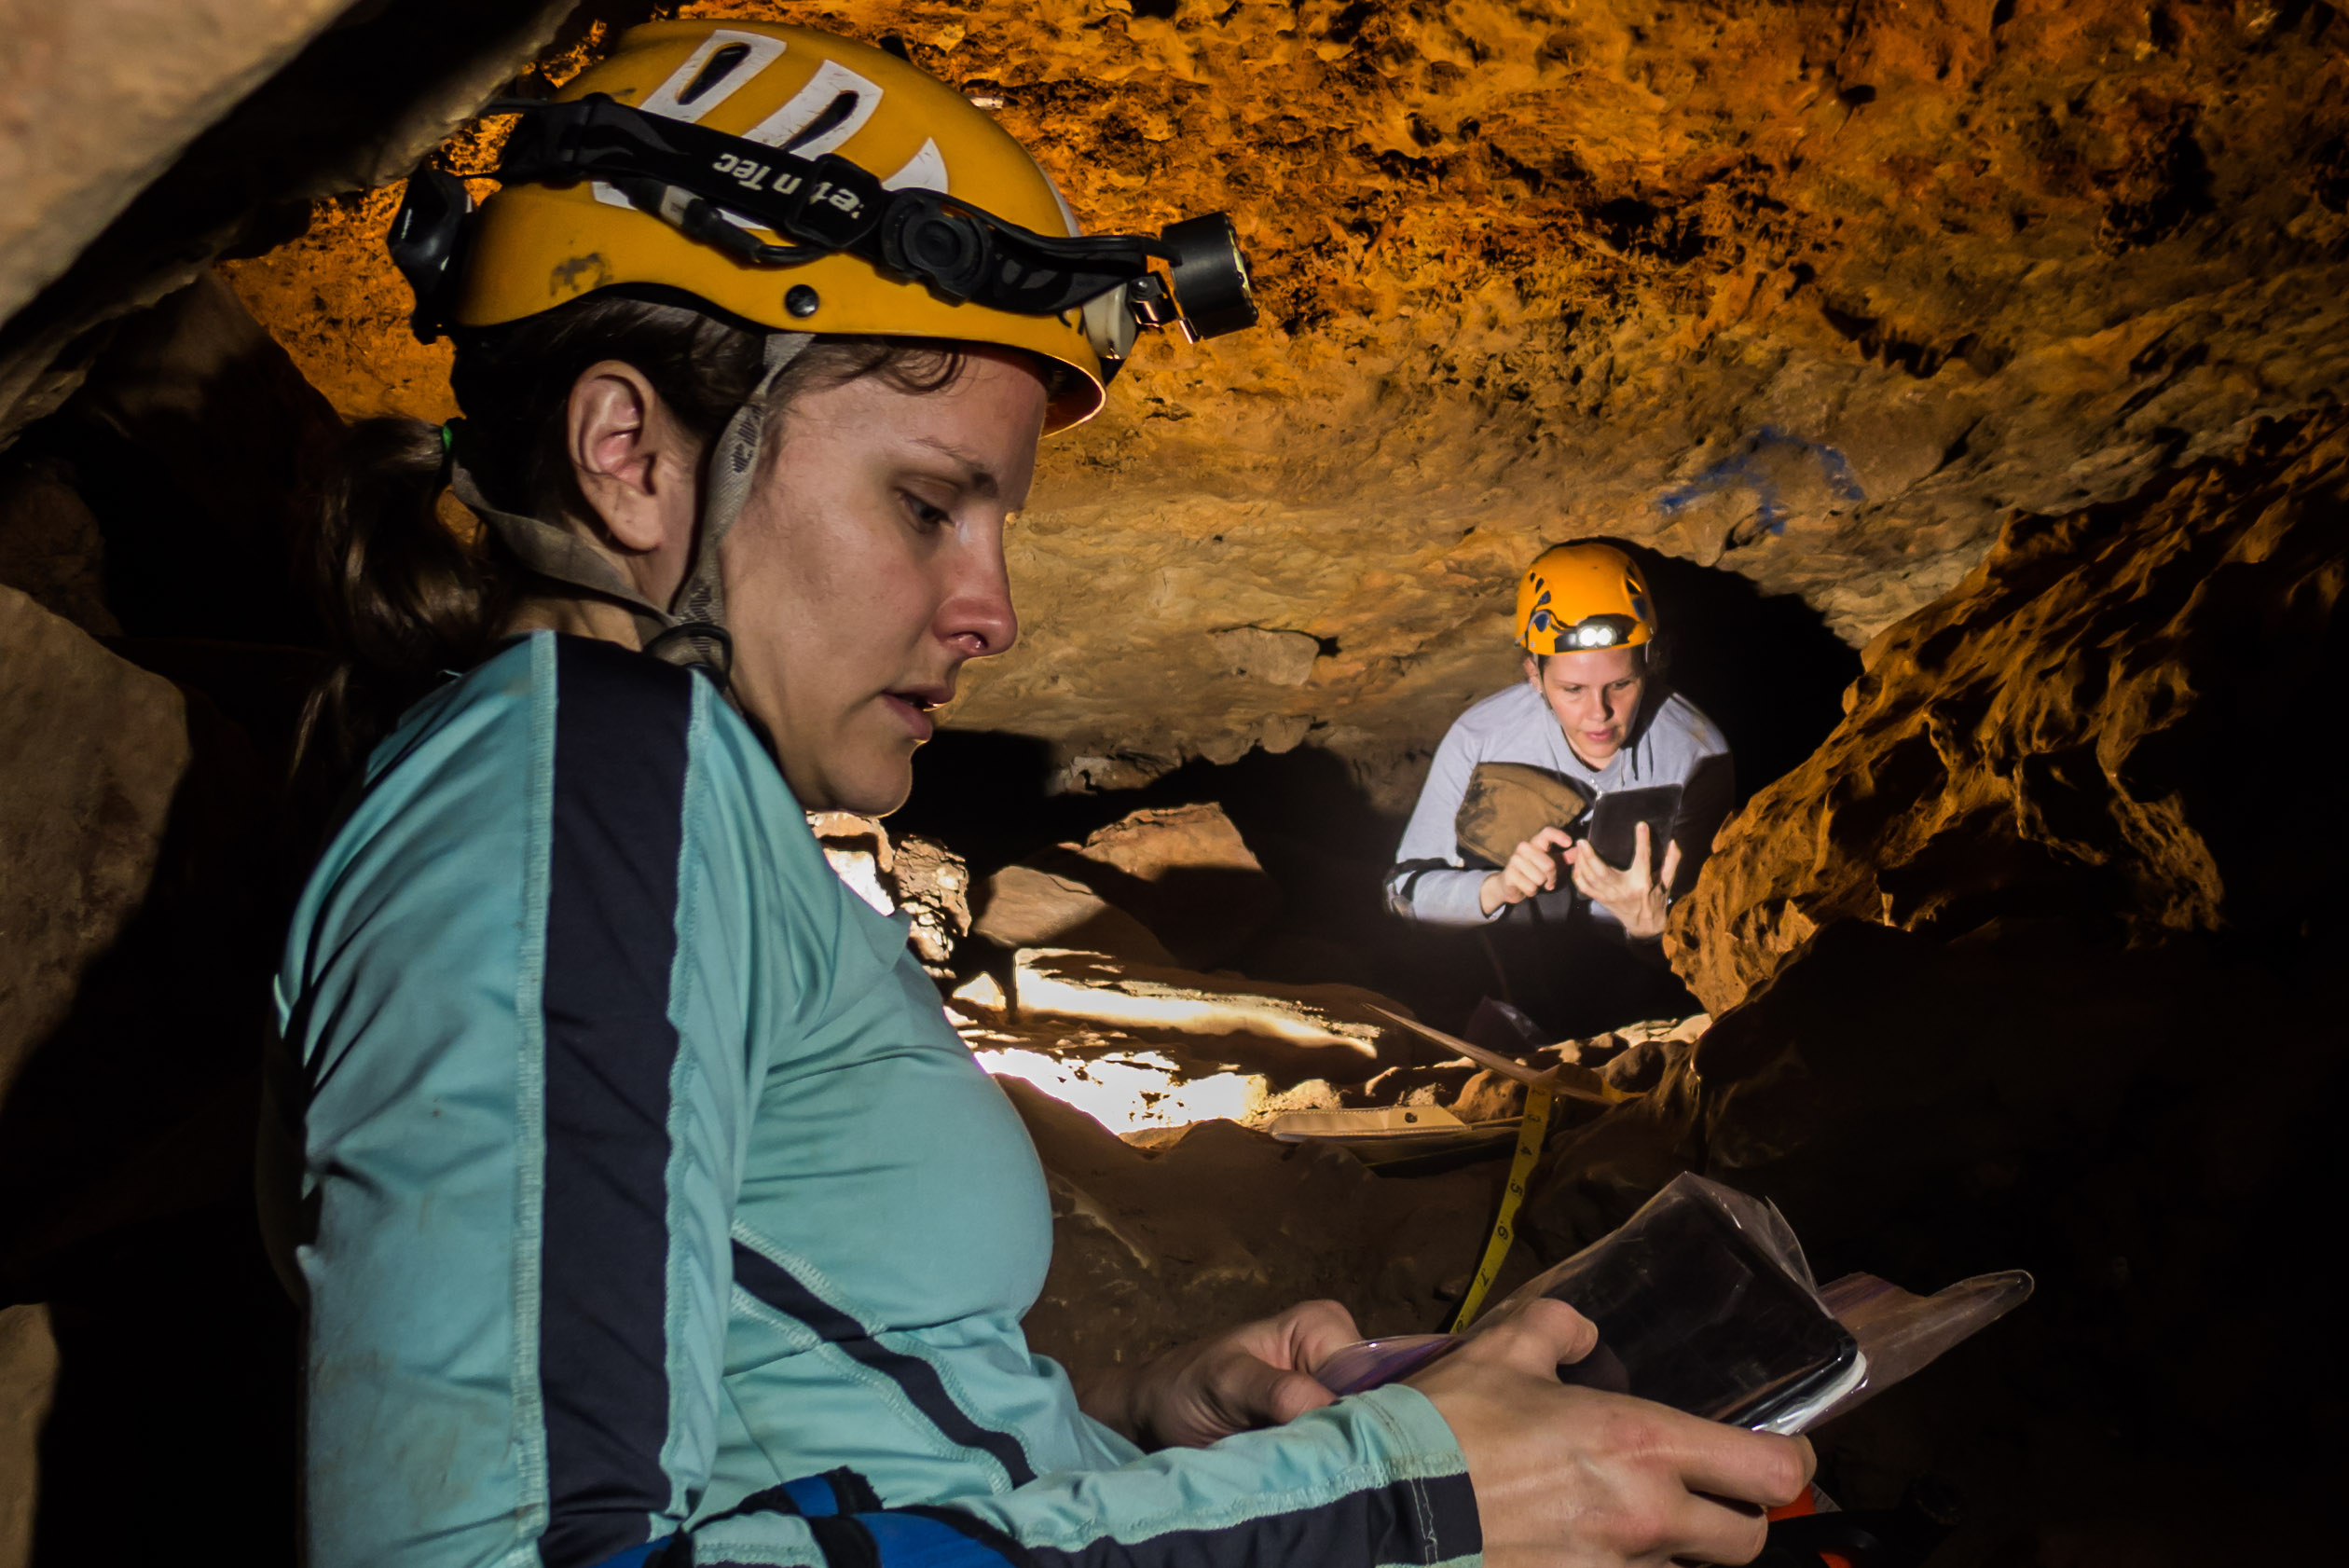
\includegraphics[width=\columnwidth]{cavewifi}
\caption{Testing WiFi Direct range in Whirlpool cave. \textit{Image courtesy of David Ochel.}}
\end{figure}

% \begin{figure}
% \includegraphics[width=\columnwidth]{whirlpool}
% \caption{Map and topology of Whirlpool cave.}
% \end{figure}

\subsection{Range Experiment Software}
\label{sec:Range Experiment Software}
An Android application was developed to perform the range experiments in a cave and to test distances that could be achieved by WiFi Direct on a mobile device.
This initial application was developed based on a WiFi Direct example provided by the Android SDK.
The example was used to learn how to create the necessary WiFi Direct components, and understand how the significant asynchronous function calls operate together.
To perform the range experiments the example was modified to open a connection to a single device, load a data file from the device, and send the data file. 
The original application provided the ability for the client to launch the other device's photo gallery and select a photo to be copied.
This functionality was removed for the purposes of our experiment, and replaced with functionality that would allow us to transfer a true sample data file from a data logger.

The Android application followed the architecture described in Section~\ref{sec:Android APIs For WiFi Direct} for creating peer to peer connections. 
This WiFi Direct application has the ability to be either the sender or the receiver of the test data file.
The main application presents a fairly simple GUI interface allowing the user to kick off discovery of peer devices. 
Upon completion of discovery a list of available peers is displayed on the GUI.
The user can then select from the list of devices which brings up a menu to connect to that device.
Once the WiFi Direct connection is established, the user may either disconnect or select a button to transfer the data file.

After the connection is established, the device which is designated to be the receiver has slightly different functionality.
For the receiver they have the option of terminating the connection, but also have a button to allow them to reset the application to be prepared to receive the next data file.
The GUI provides the user a mechanism to take a note to be logged to the log file so that data may be captured about the test being performed at the time.
The application timestamps the start and end of the data transfer, calculates duration, and logs this information to a log file, in addition to any input the user provides from the GUI about the test.

The goal of the application was to have a means to test connectivity throughout the cave and ensure that the full data file could be transferred.
The duration of the transfer was captured as measured from one side of the connection, in the event that a benchmark was possible.
In general, the most important result provided by the application was to confirm or deny a successful file transfer.

\subsection{Data Ferry Software}
\label{sec:Data Ferry Software}
The second phase of the project was to build an Android application called SwiftDataHop, that would utilize WiFi Direct to do an automated transfer of a data logger data file across multiple mobile devices acting as a data ferry. 
This project leveraged some of the WiFi Direct data transfer code from the range software and implemented a state machine to allow the application to execute in "Operate Mode" where data hops automatically from device to device. 
To utilize Operate Mode, a configuration phase is required to identify device roles and execute WPS to store credentials.
During this project the interface to the data logger was simulated with a pre-populated data file.
The application was notified of the presence of the data file via a button click on the user interface.

SwiftDataHop has two modes of execution, Manual Mode and Operate Mode.
Manual Mode performs the same data transfer capability as was used in the range experiment software which allows WPS to be executed between device so that user intervention is not required during Operate Mode.
Manual Mode also provides a mechanism through the GUI to set device roles.
The roles that can be configured are data file initiator, a sender-receiver, and an endpoint.
A device's role is determined by whether a single upstream, a single downstream, or both an upstream and downstream device are configured.
As part of configuration in Manual Mode each device has the capability to set an upstream device, a downstream device, or both.  
A downstream device is a device from which a file is received, and an upstream device is a device to which a file is sent.
A device with no downstream device set will have the capability to initiate the file transfer of the data file in Operate Mode.
A device with both an upstream and downstream device configured will wait for a connection from a downstream device, receive a file, disconnect from the downstream device, connect to an upstream device, and then send the received file.
A device with no upstream device is an endpoint or file destination and will display the file received and location to which it is copied on the file system.
In manual mode, upstream and downstream device configuration information may be viewed.

Operate mode is the automated mode of the application.
A device cannot enter Operate mode without at least one upstream or downstream device set.
Overall the application may be in one of four states: OFF, IDLE\_WAIT, SEND\_FILE, RECEIVE\_FILE.
The OFF state means that the application is in manual mode.
When Operate Mode is entered, the device initially goes into the IDLE\_WAIT state.
There are three possible ways to transition out of the IDLE\_WAIT state.
The first, if someone clicks the button to turn Operate Mode Off, in which case the application would transition back to the OFF state.
The second if someone clicks the button to "Send File", which is only enabled on a device with only an upstream device set.
Here the application would transition to the SEND\_FILE state.
The third if a WiFi Direct Group is formed from a downstream device, in which case the device would transition into the RECEIVE\_FILE state.
If a device is in the SEND\_FILE state, after operations are performed to send the data file upstream, the device will return to the IDLE\_WAIT state.
If a device is in the RECEIVE\_FILE state, it will perform operations to receive a file, and then if an upstream device has been configured it will transition into the SEND\_FILE state.
If an upstream device has not been configured, it will transition back to the IDLE\_WAIT state as that indicates it is the final device in the transfer.

TODO: Add state machine diagram.  
The operations to send and receive a file are those required to execute WiFi Direct group formation, and once completed, to create a socket connection and perform the transfer. 
Once the send file button is clicked and a device goes into the SEND\_FILE state, it performs a WiFi Direct "Connect". 
Android APIs handle the initiation of the WiFi Direct group.
The device is notified of the successful group formation by the "onConnectionInfoAvailable" callback.
At this point a TCP socket connection to the upstream device is created using the connection info returned from the previous callback.
Once a successful connection is established, the file data is written to the socket, the socket connection is closed, and the WiFi Direct group is disconnected.
The sending device returns to the IDLE\_WAIT state.
The receiving device enters the RECEIVE\_FILE state when the "onConnectionInfoAvailable" callback is executed, meaning a downstream device has requested group formation.
The device in RECEIVE\_FILE state immediately opens a socket and waits for the downstream device to connect.
Once a connection is received, the device reads the data file from the socket, closes the socket, disconnects with WiFi Direct group.
The receiving device then either transitions to the IDLE\_WAIT state if it is an endpoint, or transitions to the SEND\_FILE state and performs send operations if it has an upstream device.

\section{Results}

\subsection{WiFi Direct Range in Open Field}
\label{sec:WiFi Direct Range in Open Field}
We found a relatively open field in north Austin to carry out some range experiments with our Nexus 7 devices.
An open field, with no line of site obstructions and no other wifi devices around, should be the most ideal setting for WiFi Direct ranges.
We started our tests at 100' apart and increased the distance by 50' to 100' at at time.
We found that our devices were easily able to connect and transfer a sample data file at distances up to 300' (91meters). 
We were able to connect and send the sample file at 350', 400', 500', and 600' (183m) with moderate success. 
At times, the connection would take longer than usual.
Also, the initial file transfer took multiple attempts.
Once the initial file was received, then subsequent transfers went much better.
However, at 650' (198m) the devices had a lot of trouble connecting, so we stopped measurements then.
This is very close to the claimed range of 200' meters.

\subsection{WiFi Direct Range in a Cave}
\label{sec:WiFi Direct Range in a Cave}
We gained access to Whirlpool Cave in south Austin with the permission of the managing entity, TCMA (http://www.tcmacaves.org/) and experimented with the range and connectivity of our Nexus 7 devices on March 16, 2014.
Whirlpool Cave is a relatively typical cave for central Texas.
It has over 400m of total passage \cite{whirlpool}. 
Most of the passages are traveled by crawling.
However, an adult can stand in some of the larger rooms.

We began our range experiments in the largest room known as Travis County room which has the longest possible horizontal line of sight available in the cave.
In this room, our device were able to easily connect and transmit test files at distances of 55', 80' and 97'. 
After 97' we were no longer able to achieve line of sight.
This distance represents nearly the maximum length of the room. 
Behind our respective survey stations, the ceiling and floor of the room quickly meet.

Next, we wanted to see how connectivity would fare in a smaller passage. 
We moved out of the Travis County room into the southerly passage known as 'B' on the map.
The height of this passage varied between 36" at the first position to 2.5' height at 28' feet distance.
We also measured a minimum height of 19" at one point in the passage between survey stations.
This passage is a few meters wide per the map, so we did not specifically measure that dimension as height was the limiting factor.
Our Nexus devices successfully connected at 8' and 28' feet apart.
After 28' apart, the passage starts to turn making line of sight was impossible to maintain, so our devices could not connect.
Furthermore, since this passage was so narrow and filled with rubble, we had to take great care to maintain a line of sight between the devices.

Since the cave offers no larger rooms nor longer passages, we had to cease our experiments in Whirlpool cave at that point.
However, we suspect that in a larger cave or with straighter passages longer range should be possible.
Moore, et al carried out wifi range experiments in straight mine tunnels where they claim that signal loss attenuates there less quickly than in free space.
We refer you to that work for details.
However, we would like to state here that their work found that wifi signals attenuated less quickly in a tunnel of 8' rough diameters versus a tunnel of 15' rough diameter, so we are optimistic about the range possibilities in longer cave passages. \cite{moore2012}.


\subsection{Data Ferry Experiment Results}
\label{sec:Data Ferry Experiment Results}
Section~\ref{sec:Data Ferry Software} covered the design of the WiFi Direct data ferry application called SwiftDataHop. 

Using this prototype it was demonstrated that WiFi Direct could be used to pass data from device to device in an automated fashion. 
During the course of this project four Nexus 7 tablets running Android 4.4.2 were tested and could successfully execute the transfer.
The project was limited to four devices simply by the number of available tablets.
In theory additional devices could be added to achieve further distances or deal with larger number of topology challenges in the cave that could prevent line of sight connectivity. 
While the SwiftDataHop application was able to execute the automated transfer across four devices, there are still several issues that would need to be resolved before the application could be put to practical use.
Timing was a key challenge in implementing the Operate Mode, or automated mode, of this application.
The application was tuned for our experiment with delays to allow for connection time, disconnect time, and file transfer completion.
For example, once the first phase of creating the WiFi Direct group was completed, the sending device would receive notification that the group was established.  
Upon this notification, if the sending device opened its socket to the upstream device before the upstream device had time to open a socket and wait for connections, connectivity might fail.
Since the goal of the initial prototype was just to prove the feasibility of WiFi Direct technology in this type of application, there are likely better solutions such as implementing an acknowledgement mechanism or retries as opposed to injecting arbitrary delays into the process. 
In addition, the Android WiFi Direct APIs had some inconsistent behavior.
These APIs were very sensitive to other operations being performed on the device and offered little in terms of visibility and debug into the lower level system functions taking place on the device.
During the experiments for this project, the application could only execute a single automated transfer and then user intervention would be required to either manually disconnect from all devices, or disable and re-enable wireless services on the mobile device.
If there were additional time to dig into the source for the APIs it is highly likely that this issue could root caused and overcome.
Behavior of the APIs became more predictable when all other wireless activity was disabled on the tablets.
This would be a reasonable constraint in the cave environment as no other wireless infrastructure would be available.
In summary, this application was an effective prototype to prove that WiFi Direct could be used to leverage peer to peer connectivity in the absence of infrastructure to act as a ferry for data from in-cave loggers.

\section{Conclusions and Future Work}

\subsection{Application in Cave Systems}
\label{sec:Application in Cave Systems}
\begin{figure}

\includegraphics[width=\columnwidth]{krubera_pit_dark}
\caption{Vertical passage in Krubera-Varonya \textit{Image found in article \cite{krub_blaze}}}
\end{figure}
We performed our wifi direct experiments in a cave easily accessible to us and fairly typical of caves in this part of central Texas.
Cave systems around the world present with a wide variety of morphologies, and a given cave system will usually contain a wide variety of morphologies within it.
Morphology examples include passages that are passable only to water and insects and, in contrast, passages that are the size of large buildings and navigable by commercial aircraft.
Passages are horizontal, vertical or any angle between the two.
Some passages can be adequately described as enclosed, underground "rooms" or "pits" where the top is open to the sky.

We would like to theorize further about how our research might generalize to other caves and where this technology will have the greatest value.
WiFi Direct has several advantages including bandwidth, range, weight, and ease of deployment as we covered in Related Work, Section~\ref{sec:Related}.
However, WiFi Direct signals only work in caves when a direct line of sight is available, 
and of course the devices require a consistent source of energy.
Therefore, we propose a few example scenarios where WiFi Direct could be particularly useful as part of an in-cave communication system.

The cave Krubera-Varonya in West Caucasus in Abkhazia, Georgia is presently the world's deepest cave system with a depth of nearly 2200m and with 13.4km of passage. 
Speleologists, cavers and cave divers have been exploring and mapping this cave since at least 1982.
Expeditions in this cave are complex operations where an example cave exploration trip will span multiple weeks with at least 19 people including cavers and cave divers.
On these expeditions, cavers will survey and map the cave, specially trained cave divers will proceed through and map underwater passages, place data loggers to measure water levels, and more.
The cavers will need to be underground for weeks at a time and stay in one or more of a handful of underground camps \cite{krub_it}.
A communication system to coordinate re-supply, logistics, and, in the worst case, coordinate a rescue operation is almost a requirement for an expedition of this magnitude.
While it is difficult to determine potential length of line of sight by looking at published photos and maps, 
it certainly seems quite possible that this cave has many passages that would be great candidates for using wifi direct.
Published photos and maps show that the cave has some very long (100m) vertical drops in large, fairly straight passages and some similarly large and long horizontal passages \cite{krub_it}.
Cavers train in specialized single rope techniques to ascend and descend such vertical passages.
Even given extensive training and experience, it takes quite a long time (multiple hours) for a team of cavers to ascend or descend long vertical drops particularly since those cavers are usually carrying very heavy gear and supplies.
Therefore, there is a great opportunity to ease the physical exertion and time burden if messages can be communicated at wifi speed and bandwidth through such a passage.
Between wifi direct points, communication could even potentially be as high fidelity as voice and video such as between the top and bottom of a particular pit.
Since this cave has several sections of very tight passage and underwater passages,
a realistic system enabling communication throughout the cave such as from camp to camp to surface would most likely need to be hybrid:
consisting of wifi direct relays wherever practical to achieve distance with ease of installation, using single wire systems in winding passages, using underwater radio signals through sump passages (only passable by trained cave divers), and so on.
In such a hybrid system, our prototype application which can automatically transfer messages from device to device would be particularly helpful.

We can envision a purely wifi direct cave communication system being used to enable communication system in certain cases such as from a pit bottom to the surface.
We can also envision wifi direct being a very important part of a hybrid system enabling communication through other extensive cave systems that are similar to Krubera-Varonya in size and complexity. 

\subsection{Future Work}
\label{sec:Future Work}
There are numerous areas that could be considered for future work that were out of scope for this project due to the time available.

During this project we did not focus on measuring or reducing power consumption.
Rather, we were focused on a showing that the WiFi Direct technology has the capability to automatically ferry data within a cave.
One reported advantage of the WiFi Direct standard over other ad hoc wireless connection standards is that it provides for better power efficiency during discovery and connect \cite{wifiwhitepaper}.
Therefore, the WiFi Direct technology is a good starting point for building a low power data ferrying solution.
However, power conservation is very important in a cave environment as access to a power source is unlikely unless the cave is a tourist cave already outfitted with a lighting system.
We propose that future work in this area can reduce power requirements beyond what is provided inherently with WiFi Direct.
For instance, the data transfer can be done with smaller, lower power devices.
One way to reduce power consumption is to minimize the human interface component.
Specifically, large screens consume a lot of power, so realistic implementations could use a smaller screen or no screen.

Another area of future research will be to better coordinate the timing of data exchange in the interests of reducing power.
For example, data transfer does not usually need to be continuous or too frequent in our target use case.
The upstream devices in our implementation do not have any way to know when a downstream device might make a connection, 
so all devices remain active at all times.
In a realistic deployment, data transfer could take place on a relatively infrequent, such as daily or weekly, basis.
Therefore, a mechanism to incorporate preprogrammed periods for the devices to be inactive
and a time schedule for all devices to awake to do a scheduled data transfer would reduce power consumption.



% - KH - I don't think this is particularly worth mentioning if we include mention of using smaller/small screen devices..
% Early in development of the data ferry application a design decision was made to drop support for smaller screened devices where the application was having difficulty rendering properly.
% This was due to code that was leveraged from the range experiment and the direction taken to implement the user interface.
% Since rendering correctly on any Android device was not a key goal of this project, the focus stayed on ensuring that the application functioned on large screen devices like the Nexus 7.


As noted in Section~\ref{sec:Data Ferry Experiment Results}, it was difficult to get the timing of operations correct in the application due to the highly asynchronous nature of the required tasks.
In the prototype, we injected preconfigured delays based on our experiments to allow time for devices to complete known longer running tasks.
A better mechanism could be to look at some sort of handshake, acknowledge, and retry design.
% (kh: unclear what is meant here, or perhaps it's covered by the above)
% There could be a better mechanism to determine that a device is in the desired state and ready before operations are executed.

We did not connect to actual data loggers in our experiments although we did use example data logger output in our experiments.
However, given that all data loggers and data storage modules provide a way to connect to another device or to the internet, 
we expect that the connection to the first ferry device should be technically possible and may be specific to the logger or storage device.
Once data has reached the final endpoint, it is accessible at the very least as a file in the device's file system.
If the final endpoint is located where wifi or cellular data is available, 
then the final device can be responsible for uploading data to the internet.
If the final endpoint is not located within wifi or cellular data range, 
then the final device will be responsible for storing accumulated data until the data is retrieved.
This final data retrieval could easily be done with WiFi Direct.

The exposure of the device to environmental issues such as dust, humidity, and water need to be considered in a practical implementation.
The Nexus 7 tablets used in this research are consumer devices and not designed for use in harsh, dirty, or wet environments.
If smaller devices are used, it will be easier to harden them to the elements.

Further work could be done to improve WiFi Direct support and reliability in middleware platforms such as Android per the issues discussed in Section~\ref{sec:Data Ferry Experiment Results}.

\section{Acknowledgements}
\label{sec:Acknowledgements}
We would like to thank David Ochel for accompanying us on our trip and for taking photos. 
We would like to thank TCMA and Matt Turner for granting access to Whirlpool Cave. 
We would also like to thank Zara Environmental for providing a sample data file
and our various friends for informally advising us on cave research needs and practices.

% \begin{figure}[!b]
%   \begin{center}
%     \includegraphics[width=3.5in]{figure.pdf}
%   \end{center}
% 
%   \caption{\small Figure caption. To get a figure to span two columns, use the environment figure* rather than figure.}
%   \label{fig-label}
% \end{figure}

\bibliographystyle{abbrv}
\bibliography{refs}
\end{document}
